\begin{center}
\begin{tabular}{ccc} \toprule
Bezeichnung & Symbol & Einheit \\ \midrule
Klemmenleistungsgewinn & $G$ &  \\
Übertragungsgewinn & $G_T$ &  \\
Verfügbarer Leistungsgewinn & $G_\text{max}$ &  \\
Zwischenfrequenz & ZF & \si{\hertz} \\
Lokaloszillatorfrequenz & $f_\text{LO}$ & \si{\hertz} \\
Eingangsleistung & $P_E$ & \si{\dBm} \\
Ausgangsleistung & $P_\text{ZF}$ & \si{\dBm} \\
Determinante S-Matrix & $\Delta_S$ & \\
Mittelpunkt Stab. für Last & $C_L$ &  \\
Radius Stab. für Last & $R_L$ &  \\
Mittelpunkt Stab. für Generator & $C_G$ &  \\
Radius Stab. für Generator & $R_G$ &  \\
\bottomrule
\end{tabular}
\end{center}


\begin{description}
\item[Gewinn von Verstärkerschaltungen] \todo{überprüfen, siart}
\begin{align*}
%G &= \frac{\text{Leistung an die Last}}{\text{Leistung vom Generator}} = \\
%&= \frac{\vert S_{21}(1-|r_L|^2)\vert^2}{1- |S_{11}|^2 + |r_L|^2 (|S_{11}|^2 - |\Delta_S|^2) -2\Re\{r_L(S_{22} - S_{11}^* \Delta_S) \}} \\
%G_T &= \frac{\text{Leistung an die Last}}{\text{Vom Generator verfügbare Leistung}} = \\
%&= \frac{1 - |r_G|^2}{|1-r_G S_{11}|^2} \frac{1 - |r_L|^2}{|1-r_L r_2^2|} \\
G_\text{max} &= \frac{\text{Vom Verstärker verfügbare Leistung}}{\text{Vom Generator verfügbare Leistung}} = \\
&=  \frac{|S_{21}|^2}{(1-|S_{11}|^2)(1-|S_{22}|^2)} \qquad \textit{bei Leistungsanpassung}
\end{align*}
\item[Stabilität von Verstärkerschaltungen]
\begin{align*}
C_L &= \frac{(S_{22}-\Delta_S S_{11}^*)^*}{|S_{22}|^2 - |\Delta_S|^2} \\
R_L &= \left\vert \frac{S_{12}S_{21}}{|S_{22}|^2 - |\Delta_S|^2} \right\vert \\
C_G &= \frac{(S_{11}-\Delta_S S_{22}^*)^*}{|S_{11}|^2 - |\Delta_S|^2} \\
R_G &= \left\vert \frac{S_{21}S_{12}}{|S_{11}|^2 - |\Delta_S|^2} \right\vert \\
K &= \frac{1 - |S_{11}|^2 - |S_{22}|^2 + |\Delta_S|^2}{2|S_{12}||S_{21}|}\\
\end{align*}
Bedingungen für absolute Stabilität:
\begin{align*}
K > 1 \qquad |S_{11}| &< 1 \qquad |S_{22}| < 1 \\
|S_{12}S_{21}| &< 1-|S_{22}|^2 \\
|S_{12}S_{21}| &< 1-|S_{11}|^2 \\
\end{align*}
Bedingt stabil, wenn Stabilitätskreise den Rand des SD schneiden.

\item[Mischer] Kann ein Signal auf eine andere Frequenz (ZF) verschieben, erzeugt aber wegen Nichtlinearität Nebenprodukte, die nachträglich gefiltert werden müssen, sowohl vor als auch nach dem Mischer.
\begin{center}
\begin{tikzpicture}[scale=0.4, every node/.style={scale=0.7}]
\draw (0,0) rectangle +(3,3) node[midway] {Mischer};
\draw[-o] (1.5,3)--+(0,2) node[left,xshift=-0.04cm] {LO};
\draw[-o] (0,1.5)--+(-2,0) node[below,yshift=-0.1cm] {$f$};
\draw[-o] (3,1.5)--+(2,0) node[below,yshift=-0.1cm] {$f_\text{ZF}$};
\end{tikzpicture}
\end{center}
\begin{center}
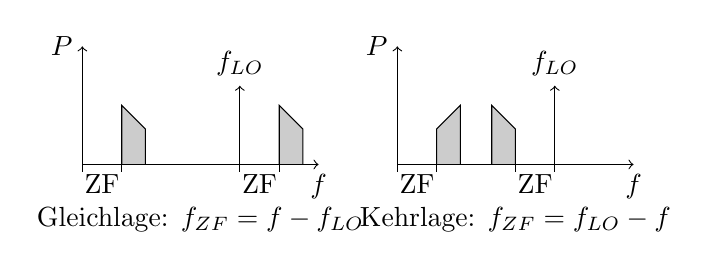
\begin{tikzpicture}[scale=1, every node/.style={scale=1}]
\def\y{1.5};
\def\x{3};

\begin{scope}
\draw[->] (\x ,0) ++(-1,0) --++(0,\y -0.5) node [above] {$f_\text{LO}$};
\filldraw[color=black,fill=black!20] (\x ,0) ++(-0.5,0)--++(0,\y -0.75)--++(0.3,-0.3)--++(0,-0.45);
\draw[|-|] (\x ,0) ++(-1.008,0)--++(0.516,0) node [midway,below] {ZF};


\filldraw[color=black,fill=black!20] ++(0.5,0)--++(0,\y -0.75)--++(0.3,-0.3)--++(0,-0.45);
\draw[|-|] (-0.006,0)--++(0.513,0) node [midway,below] {ZF};

\draw[<->] (0,\y) node[left] {$P$} -- (0,0) --  (\x ,0) node[below] {$f$};

\draw (\x /2,-0.7) node{Gleichlage: $f_\text{ZF} = f - f_\text{LO}$};
\end{scope}

\begin{scope}[xshift=4cm]
\draw[->] (\x ,0) ++(-1,0) --++(0,\y -0.5) node [above] {$f_\text{LO}$};
\filldraw[color=black,fill=black!20] (\x ,0) ++(-1.8,0)--++(0,\y -0.75)--++(0.3,-0.3)--++(0,-0.45);
\draw[|-|] (\x ,0) ++(-1.508,0)--++(0.516,0) node [midway,below] {ZF};


\filldraw[color=black,fill=black!20] ++(0.5,0)--++(0,\y -1.05)--++(0.3,00.3)--++(0,-0.75);
\draw[|-|] (-0.006,0)--++(0.513,0) node [midway,below] {ZF};

\draw[<->] (0,\y) node[left] {$P$} -- (0,0) --  (\x ,0) node[below] {$f$};
\draw (\x /2,-0.7) node{Kehrlage: $f_\text{ZF} = f_\text{LO} - f$};
\end{scope}
\end{tikzpicture}
\end{center}
Der Dynamikbereich eines Mischers wird durch das Heraustreten der Intermodulationsprodukte 3. Art aus dem Rauschen definiert, der Punkt $\text{IP}_3$ ist der Schnittpunkt der linearisierten Leistungskennlinie und die der $\text{IP}_3$-Kennlinie. Der 1-dB-Kompressionspunkt ist der Punkt, an dem die linearisierte Kennlinie um \SI{1}{\dB} von ihrem echten Verlauf abweicht (Sättigung).
\begin{center}
\begin{tikzpicture}[scale=1, every node/.style={scale=1}]
\def\y{4};
\def\x{6};

\filldraw[pattern=crosshatch,pattern color=black!10, draw=white] (0,0) rectangle +(\x-0.5,1);

\filldraw[color=green] (0.5,0) rectangle +(1.85,1);
\draw (1.4,-0.3) node {Dynamikbereich};
\draw (4.5,0.5) node {Rauschen};

\draw (0,0.5) --++(2,2)--++(0.1,0.09)--++(0.1,0.08)--++(0.1,0.07)--++(0.1,0.06)--++(0.1,0.06)--++(0.1,0.05)--++(0.1,0.04)--++(0.1,0.03)--++(0.1,0.02) --++(1,0.1) --++(1,0.01);
\draw[style=dashed] (2,2.5)--++(1.5,1.5);
\draw (2,0) --++(1.3333,4);

\draw (1,1.5)--++(0.75,0) node[below,midway] {1} --++(0,0.75) node[right,midway] {1};
\draw (2.5,1.5)--++(0.333,0) node[below,midway] {1}--++(0,1) node[right,midway] {3};

\filldraw[color=black] (3.25,3.75) circle (0.1) +(0.1,0) node [right] {$\text{IP}_3$};

\draw[|-|] (2.7,2.95)--++(0,0.25) node[left] {1dB-Komp.punkt};

\draw[<->] (0,\y) node[left] {$P_\text{ZF}$} -- (0,0) --  (\x ,0) node[below] {$P_E$};

\end{tikzpicture}
\end{center}
\end{description}